An amplifier has a dc gain of $10^5$ and poles at $10^5$ Hz , $3.16 \times 10^5$ Hz and $10^6$ Hz . Find the value of $\beta$,and the corresponding closed-loop gain , for which a phase margin of $45\degree$ is obtained. 

\begin{enumerate}[label=\arabic*.,ref=\theenumi]
\numberwithin{equation}{enumi}

\item Find the transfer function of the three pole OPAMP.
\\
\solution 
For a 3-pole amplifier open loop transfer function is 
\begin{align}
G(s) = \frac{G_0}{\brak{1+\frac{s}{P_{1}}}\brak{1+\frac{s}{P_{2}}}\brak{1+\frac{s}{P_{3}}}}
\end{align}

where the Gain and Poles are listed in Table \ref{table:ee18btech11016_Table_1}.
%
\begin{table}[!ht]
\centering


%%  This section checks if we are begin input into another file or  %%
%%  the file will be compiled alone. First use a macro taken from   %%
%%  the TeXbook ex 7.7 (suggestion of Han-Wen Nienhuys).            %%
\def\ifundefined#1{\expandafter\ifx\csname#1\endcsname\relax}


%%  Check for the \def token for inputed files. If it is not        %%
%%  defined, the file will be processed as a standalone and the     %%
%%  preamble will be used.                                          %%
\ifundefined{inputGnumericTable}

%%  We must be able to close or not the document at the end.        %%
	\def\gnumericTableEnd{\end{document}}


%%%%%%%%%%%%%%%%%%%%%%%%%%%%%%%%%%%%%%%%%%%%%%%%%%%%%%%%%%%%%%%%%%%%%%
%%                                                                  %%
%%  This is the PREAMBLE. Change these values to get the right      %%
%%  paper size and other niceties.                                  %%
%%                                                                  %%
%%%%%%%%%%%%%%%%%%%%%%%%%%%%%%%%%%%%%%%%%%%%%%%%%%%%%%%%%%%%%%%%%%%%%%

	\documentclass[12pt%
			  %,landscape%
                    ]{report}
       \usepackage[latin1]{inputenc}
       \usepackage{fullpage}
       \usepackage{color}
       \usepackage{array}
       \usepackage{longtable}
       \usepackage{calc}
       \usepackage{multirow}
       \usepackage{hhline}
       \usepackage{ifthen}
%%  End of the preamble for the standalone. The next section is for %%
%%  documents which are included into other LaTeX2e files.          %%
\else

%%  We are not a stand alone document. For a regular table, we will %%
%%  have no preamble and only define the closing to mean nothing.   %%
    \def\gnumericTableEnd{}

%%  If we want landscape mode in an embedded document, comment out  %%
%%  the line above and uncomment the two below. The table will      %%
%%  begin on a new page and run in landscape mode.                  %%
%       \def\gnumericTableEnd{\end{landscape}}
%       \begin{landscape}


%%  End of the else clause for this file being \input.              %%
\fi

%%%%%%%%%%%%%%%%%%%%%%%%%%%%%%%%%%%%%%%%%%%%%%%%%%%%%%%%%%%%%%%%%%%%%%
%%                                                                  %%
%%  The rest is the gnumeric table, except for the closing          %%
%%  statement. Changes below will alter the table's appearance.     %%
%%                                                                  %%
%%%%%%%%%%%%%%%%%%%%%%%%%%%%%%%%%%%%%%%%%%%%%%%%%%%%%%%%%%%%%%%%%%%%%%

\providecommand{\gnumericmathit}[1]{#1} 
%%  Uncomment the next line if you would like your numbers to be in %%
%%  italics if they are italizised in the gnumeric table.           %%
%\renewcommand{\gnumericmathit}[1]{\mathit{#1}}
\providecommand{\gnumericPB}[1]%
{\let\gnumericTemp=\\#1\let\\=\gnumericTemp\hspace{0pt}}
 \ifundefined{gnumericTableWidthDefined}
        \newlength{\gnumericTableWidth}
        \newlength{\gnumericTableWidthComplete}
        \newlength{\gnumericMultiRowLength}
        \global\def\gnumericTableWidthDefined{}
 \fi
%% The following setting protects this code from babel shorthands.  %%
 \ifthenelse{\isundefined{\languageshorthands}}{}{\languageshorthands{english}}
%%  The default table format retains the relative column widths of  %%
%%  gnumeric. They can easily be changed to c, r or l. In that case %%
%%  you may want to comment out the next line and uncomment the one %%
%%  thereafter                                                      %%
\providecommand\gnumbox{\makebox[0pt]}
%%\providecommand\gnumbox[1][]{\makebox}

%% to adjust positions in multirow situations                       %%
\setlength{\bigstrutjot}{\jot}
\setlength{\extrarowheight}{\doublerulesep}

%%  The \setlongtables command keeps column widths the same across  %%
%%  pages. Simply comment out next line for varying column widths.  %%
\setlongtables

\setlength\gnumericTableWidth{%
	60pt+%
	100pt+%
0pt}
\def\gumericNumCols{2}
\setlength\gnumericTableWidthComplete{\gnumericTableWidth+%
         \tabcolsep*\gumericNumCols*2+\arrayrulewidth*\gumericNumCols}
\ifthenelse{\lengthtest{\gnumericTableWidthComplete > \linewidth}}%
         {\def\gnumericScale{\ratio{\linewidth-%
                        \tabcolsep*\gumericNumCols*2-%
                        \arrayrulewidth*\gumericNumCols}%
{\gnumericTableWidth}}}%
{\def\gnumericScale{1}}

%%%%%%%%%%%%%%%%%%%%%%%%%%%%%%%%%%%%%%%%%%%%%%%%%%%%%%%%%%%%%%%%%%%%%%
%%                                                                  %%
%% The following are the widths of the various columns. We are      %%
%% defining them here because then they are easier to change.       %%
%% Depending on the cell formats we may use them more than once.    %%
%%                                                                  %%
%%%%%%%%%%%%%%%%%%%%%%%%%%%%%%%%%%%%%%%%%%%%%%%%%%%%%%%%%%%%%%%%%%%%%%

\ifthenelse{\isundefined{\gnumericColA}}{\newlength{\gnumericColA}}{}\settowidth{\gnumericColA}{\begin{tabular}{@{}p{60pt*\gnumericScale}@{}}x\end{tabular}}
\ifthenelse{\isundefined{\gnumericColB}}{\newlength{\gnumericColB}}{}\settowidth{\gnumericColB}{\begin{tabular}{@{}p{100pt*\gnumericScale}@{}}x\end{tabular}}
\begin{tabular}[c]{%
	b{\gnumericColA}%
	b{\gnumericColB}%%
	}

%%%%%%%%%%%%%%%%%%%%%%%%%%%%%%%%%%%%%%%%%%%%%%%%%%%%%%%%%%%%%%%%%%%%%%
%%  The longtable options. (Caption, headers... see Goosens, p.124) %%
%	\caption{The Table Caption.}             \\	%
% \hline	% Across the top of the table.
%%  The rest of these options are table rows which are placed on    %%
%%  the first, last or every page. Use \multicolumn if you want.    %%

%%  Header for the first page.                                      %%
%	\multicolumn{3}{c}{The First Header} \\ \hline 
%	\multicolumn{1}{c}{colTag}	%Column 1
%	&\multicolumn{1}{c}{colTag}	%Column 2
%	&\multicolumn{1}{c}{colTag}	\\ \hline %Last column
%	\endfirsthead

%%  The running header definition.                                  %%
%	\hline
%	\multicolumn{3}{l}{\ldots\small\slshape continued} \\ \hline
%	\multicolumn{1}{c}{colTag}	%Column 1
%	&\multicolumn{1}{c}{colTag}	%Column 2
%	&\multicolumn{1}{c}{colTag}	\\ \hline %Last column
%	\endhead

%%  The running footer definition.                                  %%
%	\hline
%	\multicolumn{3}{r}{\small\slshape continued\ldots} \\
%	\endfoot

%%  The ending footer definition.                                   %%
%	\multicolumn{3}{c}{That's all folks} \\ \hline 
%	\endlastfoot
%%%%%%%%%%%%%%%%%%%%%%%%%%%%%%%%%%%%%%%%%%%%%%%%%%%%%%%%%%%%%%%%%%%%%%

\hhline{|-|-}
	 \multicolumn{1}{|p{\gnumericColA}|}%
	{\gnumericPB{\centering}\textbf{Parameters}}
	&\multicolumn{1}{p{\gnumericColB}|}%
	{\gnumericPB{\centering}\textbf{Value}}

	
\\


\hhline{|--|}
	 \multicolumn{1}{|p{\gnumericColA}|}%
	{\gnumericPB{\centering}$P_{1}$}
	&\multicolumn{1}{p{\gnumericColB}|}%
	{\gnumericPB{\centering}$2\pi\times10^{5}$ rad/sec}


\\


\hhline{|--|}
	 \multicolumn{1}{|p{\gnumericColA}|}%
	{\gnumericPB{\centering}$P_{2}$}
	&\multicolumn{1}{p{\gnumericColB}|}%
	{\gnumericPB{\centering}$2\pi(3.16\times10^{5})$ rad/sec}


\\

\hhline{|--|}
	 \multicolumn{1}{|p{\gnumericColA}|}%
	{\gnumericPB{\centering}$P_{3}$}
	&\multicolumn{1}{p{\gnumericColB}|}%
	{\gnumericPB{\centering}$2\pi\times10^{6}$ rad/sec}


\\



\hhline{|--|}
	 \multicolumn{1}{|p{\gnumericColA}|}%
	{\gnumericPB{\centering}$G_0$}
	&\multicolumn{1}{p{\gnumericColB}|}%
	{\gnumericPB{\centering}$10^{5}$}



\\
\hhline{|-|-|}
\end{tabular}

\ifthenelse{\isundefined{\languageshorthands}}{}{\languageshorthands{\languagename}}
\gnumericTableEnd


\caption{}
\label{table:ee18btech11016_Table_1}
\end{table}

Poles are at $f_{1} =10^5$ and $f_{2} = 3.16\times10^{5}$ and $f_{3} = 10^6$ 
\begin{multline}
G\brak{f} = \frac{G_{0}}{\brak{1+\j\frac{f}{f_{1}}}\brak{1+\j\frac{f}{f_{2}}}\brak{1+\j\frac{f}{f_{3}}}}\\
= \frac{10^{5}}{\brak{1+\j\frac{f}{10^5}}\brak{1+\j\frac{f}{3.16\times10^{5}}}\brak{1+\j\frac{f}{10^6}}}
\label{eq:ee18btech11016_1}
\end{multline}
\item Find the loop gain expression ($G(s)H$) (H is constant in this question).
\\
\solution 
\begin{align}
GH = \frac{10^{5}}{\brak{1+\j\frac{f}{10^5}}\brak{1+\j\frac{f}{3.16\times10^{5}}}\brak{1+\j\frac{f}{10^6}}} . H
\label{eq:ee18btech11016_2}
\end{align}

\item Find the PM and the crossover frequency.
\\
\solution  
The phase margin = $180\degree$ - $\phi(f_{c})$ where $f_{c}$ is the frequency where $\abs{G(f)H}=1$.It is required that the phase margin is $45\degree$ , so that :

\begin{align}
45\degree &=  180\degree - \phi(f_{c}) \implies \phi(f_{c})=-135\degree.
\end{align}
From \eqref{eq:ee18btech11016_2} 
\begin{align}
-135\degree = -\tan^{-1}\brak{\frac{f_{c}}{10^5}}-\tan^{-1}\brak{\frac{f_{c}}{3.16\times10^5}}-\tan^{-1}\brak{\frac{f_{c}}{10^6}}
\end{align}
After solving the above equation , we get $f_{c}$ = 315KHz.
\\

\item Verify your result using a Bode plot.
\\
\solution  The following code  id used to verify the value of $f_{c}$ Fig. \ref{fig:ee18btech11016_1}

\begin{lstlisting}
codes/ee18btech11016/ee18btech11016_1.py
\end{lstlisting}
%
\begin{figure}[!h]
\centering
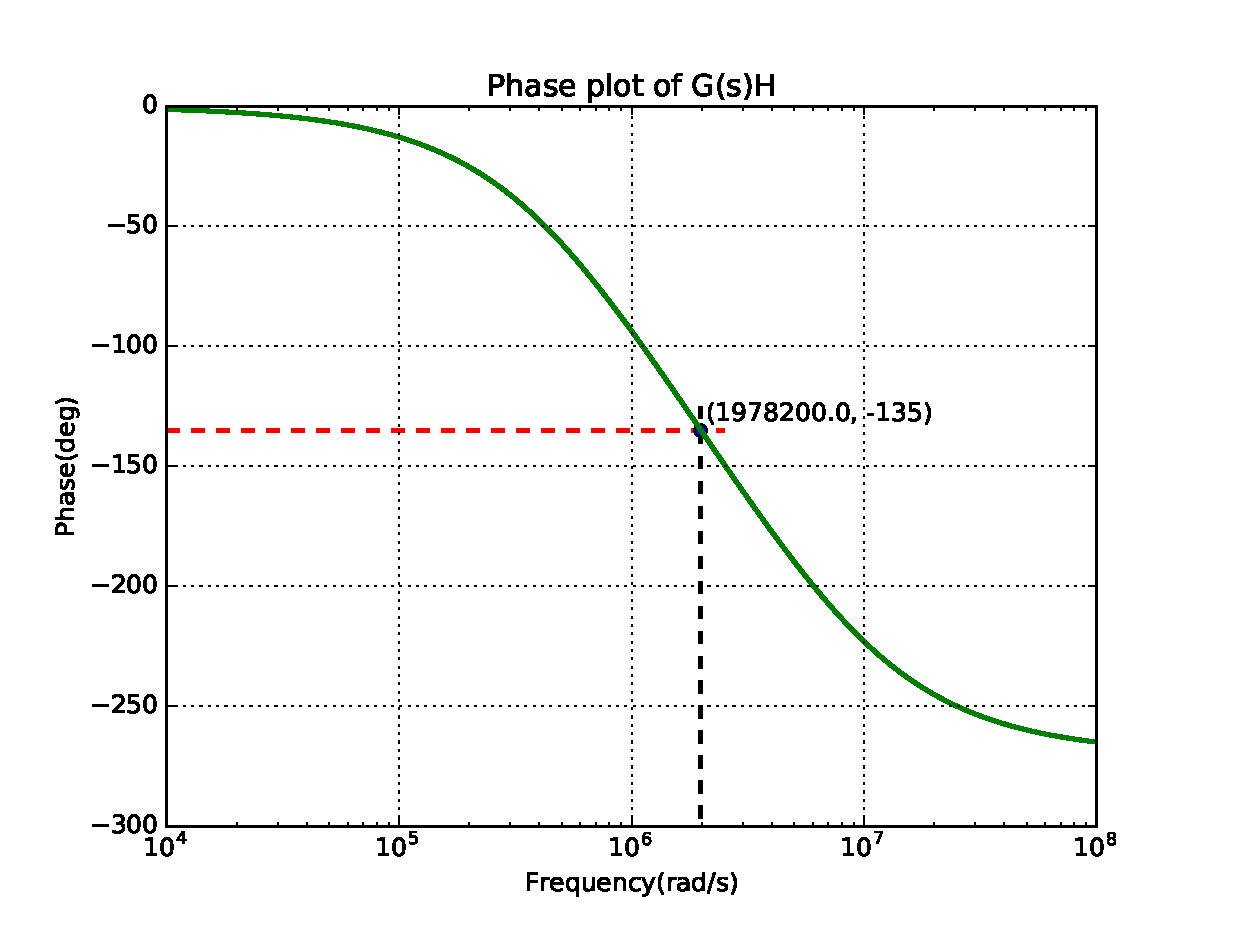
\includegraphics[width=\columnwidth]{./figs/ee18btech11016/ee18btech11016_resultbode.eps}
\caption{}
\label{fig:ee18btech11016_1}
\end{figure}

\item Find the value of H.\\
\solution From \eqref{eq:ee18btech11016_2},The magnitude of the loop gain at this frequency $f_{c}$ is given by $\abs{G(f_{c})H}$ :
 
\begin{align}
    H\brak{\frac{10^5}{\sqrt{1+(\frac{315\times10^3}{10^5})^2}\sqrt{1+(\frac{315\times10^3}{3.16\times10^6})^2}\sqrt{1+(\frac{315\times10^3}{10^6})^2}}}
\end{align}

which is equal to $H\times(28.8588\times10^3)$.
So,
\begin{align}
\abs{G(f_{c})H} = H\times(28.8588\times10^3)
\end{align}

Setting $\abs{G(f_{c})H}$ = 1 , Solving for $\beta$ (here $\beta$ is equal to H) yields 
\begin{align}
\beta &= 34.651\times10^{-6}
\end{align}
Or
\begin{align}
H &= 34.651\times10^{-6}
\end{align}

The following code provides the method to calculate the unit step response and the values of H,G(fc).
\begin{lstlisting}
codes/ee18btech11016/ee18btech11016_verifyingvalues.py
\end{lstlisting}
\item Find the corresponding closed-loop gain for which a phase margin of $45\degree$ is obtained.\\
\solution The closed loop dc gain is given as
\begin{align}
A_{f} = \frac{G_{0}}{1+HG_{0}}=\frac{10^5}{1+34.651\times10^{-6}(10^5)}
\end{align} 
\begin{align}
A_{f} = 22.3957\times10^3
\end{align}


\item Realise the above system with $PM = 45 \degree$ using a feedback circuit.\\
\solution
\begin{figure}[ht!]
	\begin{center}
		\resizebox{\columnwidth/1}{!}{\tikzstyle{block} = [draw, rectangle, 
    minimum height=1.25em, minimum width=2.5em]
\tikzstyle{sum} = [draw, circle, node distance=1cm]
\tikzstyle{input} = [coordinate]
\tikzstyle{output} = [coordinate]
\tikzstyle{pinstyle} = [pin edge={to-,thin,black}]

% The block diagram code is probably more verbose than necessary
\begin{tikzpicture}[auto, node distance=2.5cm,>=latex']
    % We start by placing the blocks
    \node [input, name=input] {};
    \node [sum, right of=input] (sum) {};
    \node [block, right of=sum] (controller) {$G(s)$};
    
    % We draw an edge between the controller and system block to 
    % calculate the coordinate u. We need it to place the measurement block. 
   
    \node [output, right of=controller] (output) {};
    \node [block, below of=controller] (measurements) {$48.9\times10^{-6}$};

    % Once the nodes are placed, connecting them is easy. 
    \draw [draw,->] (input) -- node[pos=0.99] {$+$} node {$V_{s}$} (sum);
    \draw [->] (sum) -- node {$V_{i}$} (controller);
    \draw [->] (controller) -- node [name=y] {$V_{o}$}(output);
    \draw [->] (y) |- (measurements);
    \draw [->] (measurements) -| node[pos=0.99] {$-$} node [near end] {$V_{f}$} (sum);
\end{tikzpicture}}
	\end{center}
	\caption{}
	\label{fig:ee18btech11016_figa}
\end{figure}

The transfer function of OPAMP is
\begin{align}
    G(s) = \frac{10^{5}}{\brak{1+\frac{s}{2\pi \times 10^5}}\brak{1+\frac{s}{2\pi \times3.16 \times 10^{5}}}\brak{1+\frac{s}{2\pi \times 10^{6}}}}
\end{align}
%
\item For the feedback gain H\\
\solution\\
Choose a resistance network such that
\begin{align}
    H = \frac{V_{f}}{V_{o}} = \frac{R_{f_{1}}}{R_{f_{1}}+R_{f_{2}}} \approx 34.651\times10^{-6}
\end{align}
\begin{figure}[ht!]
	\begin{center}
		\resizebox{\columnwidth/2}{!}{\begin{circuitikz}[american]
\ctikzset{tripoles/mos style/arrows}
\draw (1,2) to[short, -o] (0,2) node[label={below:$v_{o}$}]{};
\draw (1,2) to[R=$R_{f_{2}}$] (2,2) -- (3,2) to[R=$R_{f_{1}}$] (3,0) node[ground](GND){};
\draw (3,2) to[short, -o] (4,2) node[label={below:$v_{f}$}]{};
\end{circuitikz}}
	\end{center}
	\caption{}
	\label{fig:ee18btech11016_figb}
\end{figure}

Choose $R_{f_{1}}$ and $R_{f_{2}}$ as
\begin{align}
    R_{f_{1}} = 100\ohm\\
    R_{f_{2}} = 4.057M\ohm
\end{align}
\begin{align}
H = \frac{R_{f_{1}}}{R_{f_{1}}+R_{f_{2}}} = \frac{100}{100+4.057\times10^6} \approx 34.651\times10^{-6}
\end{align}
\item Feedback Circuit for $PM = 45\degree$
\\
\solution
\begin{figure}[ht!]
	\begin{center}
		\resizebox{\columnwidth}{!}{\begin{circuitikz}[american]

\draw (2,2)  node[op amp] (OA) {};
\draw (OA.+) -- (0,1.5) to[vsourcesin, l= $V_{s}$] (0,0) node[ground](GND){};
\draw (OA.-) -- (0,2.5) node[label={below:$V_{f}$}]{} to[R,l_=$100\ohm$] (-2,2.5) node[ground](GND){};
\draw (OA.out) -- (3,2) node[label={}]{};
\draw (3,2) -- (4.5,2) node[label={above:$V_{o}$}]{};
%\draw (3,2) to[R=$5300\ohm$] (5.5,2) node[label={}]{} to[C,l_=$3nF$] (5.5,0) node[ground](GND){};
%\draw (5.5,2) -- (6.5,2) node[label={above:$V_{o}$}]{};
\draw (3,2) -- (3,4.5) to[R=$4.057M\ohm$] (0,4.5) -- (0,2.5);
\end{circuitikz}
}
	\end{center}
	\caption{}
	\label{fig:ee18btech11016_figc}
\end{figure}

\item Simulate the circuit in ngspice.\\
\solution For $H=34.651\times10^{-6}$ the closed loop response is
\begin{align}
\abs T \approx \frac{1}{H} = 28.8588\times10^{3}
\end{align}
which can be observable from graph also.
\\

The following code provides instructions about the simulation.
\begin{lstlisting}
codes/ee18btech11016/spice/README.md
\end{lstlisting}


The following netlist simulates the unity feedback system. 
\\

\begin{lstlisting}
codes/ee18btech11016/spice/ee18btech1016_sim.net
\end{lstlisting}
 The step response in spice is plotted using the following code in Fig. \ref{fig:ee18btech11016_spice}
 \begin{lstlisting}
codes/ee18btech11016/spice/ee18btech11016_simulation.py
\end{lstlisting}
\begin{figure}[!h]
\centering
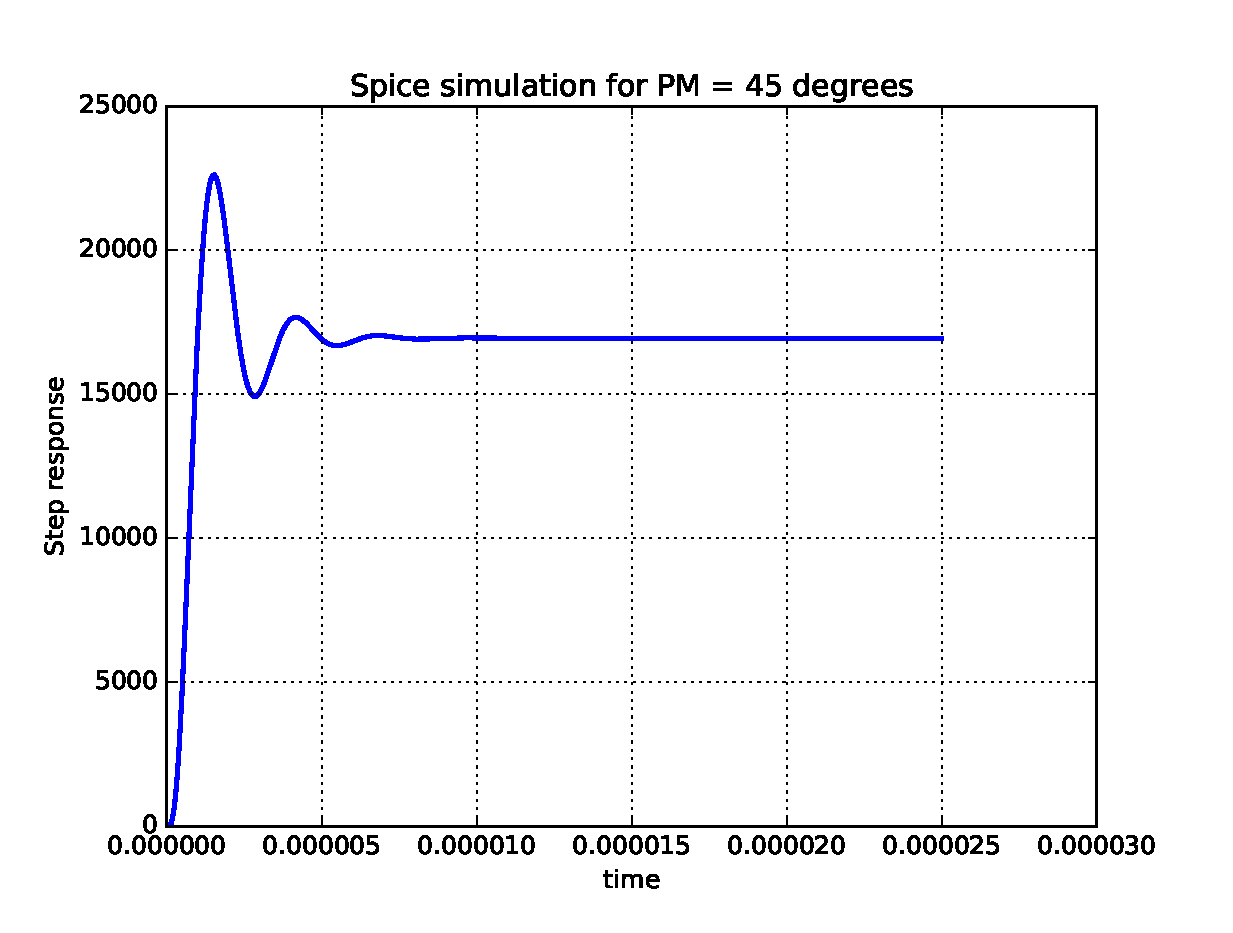
\includegraphics[width=\columnwidth]{./figs/ee18btech11016/ee18btech11016_spice.eps}
\caption{}
\label{fig:ee18btech11016_spice}
\end{figure}

\item Overview of implementation.\\
\solution Fig. \ref{fig:ee18btech110016_circuit_1} shows how the circuit is actually implemented in spice using the parameters in Table \ref{table:ee18btech11016_Table_2}  

\begin{figure}[!ht]
	\begin{center}
				\resizebox{\columnwidth}{!}{
\begin{circuitikz}
\ctikzset{bipoles/length=1cm}

\draw 
(-2,1)--(-1,1)--(-1,0) to [R = $RIN$] (-1,0)--(-1,-1)--(-2,-1)


(0, 0) to[I=$ $] (0,0) to (0,-1) %node[ground]{}
(0,0) -- (0,1)--(0.25,1) to[] (1,1) 
to [R = $R_{1}$] (1,-1) 
(1,1)--(2,1)to [C = $C1$](2,-1)
(3,-1)--(3,-1.5)node[ground]{}

(4,0)to [I=$ $] (4,0) to (4,-1)
(4,0) -- (4,1)--(4.25,1) to[] (5,1)
to [R = $R_{2}$] (5,-1) 
(5,1)--(6,1)to [C = $C2$](6,-1)


(8, 0) to[I=$ $] (8,0) to (8,-1) %node[ground]{}
(8,0) -- (8,1)--(8.25,1) to[] (9,1) 
to [R = $R_{3}$] (9,-1) 
(9,1)--(10,1)to [C = $C3$](10,-1)
(0,-1)--(10,-1)

(10,-1)--(12,-1)--(12,0) --(12,1)--(12.5,1)to [R = $Rout$](14,1)

node at(-2,1.25){$V_{+}$}
node at(-2,-1.25){$V_{-}$}
node at(14,1.25){$V_{out}$}
node at(-0.25,0.65){$G1$}
node at(3.75,0.65){$G2$}
node at(7.75,0.65){$G3$}

node at(1,-1.5){$P_{1},GAIN $}
node at(5,-1.5){$P_{2} $}
node at(9,-1.5){$P_{3}$}
;\end{circuitikz}


}
	\end{center}
\caption{Circuit resembling G(s)}
\label{fig:ee18btech110016_circuit_1}
\end{figure}

\begin{table}[!ht]
\centering


%%  This section checks if we are begin input into another file or  %%
%%  the file will be compiled alone. First use a macro taken from   %%
%%  the TeXbook ex 7.7 (suggestion of Han-Wen Nienhuys).            %%
\def\ifundefined#1{\expandafter\ifx\csname#1\endcsname\relax}


%%  Check for the \def token for inputed files. If it is not        %%
%%  defined, the file will be processed as a standalone and the     %%
%%  preamble will be used.                                          %%
\ifundefined{inputGnumericTable}

%%  We must be able to close or not the document at the end.        %%
	\def\gnumericTableEnd{\end{document}}


%%%%%%%%%%%%%%%%%%%%%%%%%%%%%%%%%%%%%%%%%%%%%%%%%%%%%%%%%%%%%%%%%%%%%%
%%                                                                  %%
%%  This is the PREAMBLE. Change these values to get the right      %%
%%  paper size and other niceties.                                  %%
%%                                                                  %%
%%%%%%%%%%%%%%%%%%%%%%%%%%%%%%%%%%%%%%%%%%%%%%%%%%%%%%%%%%%%%%%%%%%%%%

	\documentclass[12pt%
			  %,landscape%
                    ]{report}
       \usepackage[latin1]{inputenc}
       \usepackage{fullpage}
       \usepackage{color}
       \usepackage{array}
       \usepackage{longtable}
       \usepackage{calc}
       \usepackage{multirow}
       \usepackage{hhline}
       \usepackage{ifthen}
%%  End of the preamble for the standalone. The next section is for %%
%%  documents which are included into other LaTeX2e files.          %%
\else

%%  We are not a stand alone document. For a regular table, we will %%
%%  have no preamble and only define the closing to mean nothing.   %%
    \def\gnumericTableEnd{}

%%  If we want landscape mode in an embedded document, comment out  %%
%%  the line above and uncomment the two below. The table will      %%
%%  begin on a new page and run in landscape mode.                  %%
%       \def\gnumericTableEnd{\end{landscape}}
%       \begin{landscape}


%%  End of the else clause for this file being \input.              %%
\fi

%%%%%%%%%%%%%%%%%%%%%%%%%%%%%%%%%%%%%%%%%%%%%%%%%%%%%%%%%%%%%%%%%%%%%%
%%                                                                  %%
%%  The rest is the gnumeric table, except for the closing          %%
%%  statement. Changes below will alter the table's appearance.     %%
%%                                                                  %%
%%%%%%%%%%%%%%%%%%%%%%%%%%%%%%%%%%%%%%%%%%%%%%%%%%%%%%%%%%%%%%%%%%%%%%

\providecommand{\gnumericmathit}[1]{#1} 
%%  Uncomment the next line if you would like your numbers to be in %%
%%  italics if they are italizised in the gnumeric table.           %%
%\renewcommand{\gnumericmathit}[1]{\mathit{#1}}
\providecommand{\gnumericPB}[1]%
{\let\gnumericTemp=\\#1\let\\=\gnumericTemp\hspace{0pt}}
 \ifundefined{gnumericTableWidthDefined}
        \newlength{\gnumericTableWidth}
        \newlength{\gnumericTableWidthComplete}
        \newlength{\gnumericMultiRowLength}
        \global\def\gnumericTableWidthDefined{}
 \fi
%% The following setting protects this code from babel shorthands.  %%
 \ifthenelse{\isundefined{\languageshorthands}}{}{\languageshorthands{english}}
%%  The default table format retains the relative column widths of  %%
%%  gnumeric. They can easily be changed to c, r or l. In that case %%
%%  you may want to comment out the next line and uncomment the one %%
%%  thereafter                                                      %%
\providecommand\gnumbox{\makebox[0pt]}
%%\providecommand\gnumbox[1][]{\makebox}

%% to adjust positions in multirow situations                       %%
\setlength{\bigstrutjot}{\jot}
\setlength{\extrarowheight}{\doublerulesep}

%%  The \setlongtables command keeps column widths the same across  %%
%%  pages. Simply comment out next line for varying column widths.  %%
\setlongtables

\setlength\gnumericTableWidth{%
	60pt+%
	90pt+%
0pt}
\def\gumericNumCols{2}
\setlength\gnumericTableWidthComplete{\gnumericTableWidth+%
         \tabcolsep*\gumericNumCols*2+\arrayrulewidth*\gumericNumCols}
\ifthenelse{\lengthtest{\gnumericTableWidthComplete > \linewidth}}%
         {\def\gnumericScale{\ratio{\linewidth-%
                        \tabcolsep*\gumericNumCols*2-%
                        \arrayrulewidth*\gumericNumCols}%
{\gnumericTableWidth}}}%
{\def\gnumericScale{1}}

%%%%%%%%%%%%%%%%%%%%%%%%%%%%%%%%%%%%%%%%%%%%%%%%%%%%%%%%%%%%%%%%%%%%%%
%%                                                                  %%
%% The following are the widths of the various columns. We are      %%
%% defining them here because then they are easier to change.       %%
%% Depending on the cell formats we may use them more than once.    %%
%%                                                                  %%
%%%%%%%%%%%%%%%%%%%%%%%%%%%%%%%%%%%%%%%%%%%%%%%%%%%%%%%%%%%%%%%%%%%%%%

\ifthenelse{\isundefined{\gnumericColA}}{\newlength{\gnumericColA}}{}\settowidth{\gnumericColA}{\begin{tabular}{@{}p{60pt*\gnumericScale}@{}}x\end{tabular}}
\ifthenelse{\isundefined{\gnumericColB}}{\newlength{\gnumericColB}}{}\settowidth{\gnumericColB}{\begin{tabular}{@{}p{90pt*\gnumericScale}@{}}x\end{tabular}}
\begin{tabular}[c]{%
	b{\gnumericColA}%
	b{\gnumericColB}%%
	}

%%%%%%%%%%%%%%%%%%%%%%%%%%%%%%%%%%%%%%%%%%%%%%%%%%%%%%%%%%%%%%%%%%%%%%
%%  The longtable options. (Caption, headers... see Goosens, p.124) %%
%	\caption{The Table Caption.}             \\	%
% \hline	% Across the top of the table.
%%  The rest of these options are table rows which are placed on    %%
%%  the first, last or every page. Use \multicolumn if you want.    %%

%%  Header for the first page.                                      %%
%	\multicolumn{3}{c}{The First Header} \\ \hline 
%	\multicolumn{1}{c}{colTag}	%Column 1
%	&\multicolumn{1}{c}{colTag}	%Column 2
%	&\multicolumn{1}{c}{colTag}	\\ \hline %Last column
%	\endfirsthead

%%  The running header definition.                                  %%
%	\hline
%	\multicolumn{3}{l}{\ldots\small\slshape continued} \\ \hline
%	\multicolumn{1}{c}{colTag}	%Column 1
%	&\multicolumn{1}{c}{colTag}	%Column 2
%	&\multicolumn{1}{c}{colTag}	\\ \hline %Last column
%	\endhead

%%  The running footer definition.                                  %%
%	\hline
%	\multicolumn{3}{r}{\small\slshape continued\ldots} \\
%	\endfoot

%%  The ending footer definition.                                   %%
%	\multicolumn{3}{c}{That's all folks} \\ \hline 
%	\endlastfoot
%%%%%%%%%%%%%%%%%%%%%%%%%%%%%%%%%%%%%%%%%%%%%%%%%%%%%%%%%%%%%%%%%%%%%%

\hhline{|-|-}
	 \multicolumn{1}{|p{\gnumericColA}|}%
	{\gnumericPB{\centering}\textbf{Elements}}
	&\multicolumn{1}{p{\gnumericColB}|}%
	{\gnumericPB{\centering}\textbf{Value}}

	
\\


\hhline{|--|}
	 \multicolumn{1}{|p{\gnumericColA}|}%
	{\gnumericPB{\centering}$G_{1}$}
	&\multicolumn{1}{p{\gnumericColB}|}%
	{\gnumericPB{\centering}$10^{-1} (V_{+} - V_{-}) A/V$}

\\


\hhline{|--|}
	 \multicolumn{1}{|p{\gnumericColA}|}%
	{\gnumericPB{\centering}$G_{2}$}
	&\multicolumn{1}{p{\gnumericColB}|}%
	{\gnumericPB{\centering}$10^{-6} A/V$}
\\


\hhline{|--|}
	 \multicolumn{1}{|p{\gnumericColA}|}%
	{\gnumericPB{\centering}$G_{3}$}
	&\multicolumn{1}{p{\gnumericColB}|}%
	{\gnumericPB{\centering}$10^{-6} A/V$}
	
\\





\hhline{|--|}
	 \multicolumn{1}{|p{\gnumericColA}|}%
	{\gnumericPB{\centering}$R_{1}$}
	&\multicolumn{1}{p{\gnumericColB}|}%
	{\gnumericPB{\centering}$1M\Omega$}
	
\\


\hhline{|--|}
	 \multicolumn{1}{|p{\gnumericColA}|}%
	{\gnumericPB{\centering}$R_{2}$}
	&\multicolumn{1}{p{\gnumericColB}|}%
	{\gnumericPB{\centering}$1M\Omega$}
	
\\


\hhline{|--|}
	 \multicolumn{1}{|p{\gnumericColA}|}%
	{\gnumericPB{\centering}$R_{3}$}
	&\multicolumn{1}{p{\gnumericColB}|}%
	{\gnumericPB{\centering}$1M\Omega$}
	
\\



\hhline{|--|}
	 \multicolumn{1}{|p{\gnumericColA}|}%
	{\gnumericPB{\centering}$C_{1}$}
	&\multicolumn{1}{p{\gnumericColB}|}%
	{\gnumericPB{\centering}$1.59pF$}
	
\\


\hhline{|--|}
	 \multicolumn{1}{|p{\gnumericColA}|}%
	{\gnumericPB{\centering}$C_{2}$}
	&\multicolumn{1}{p{\gnumericColB}|}%
	{\gnumericPB{\centering}$0.503pF$}
	
\\


\hhline{|--|}
	 \multicolumn{1}{|p{\gnumericColA}|}%
	{\gnumericPB{\centering}$C_{3}$}
	&\multicolumn{1}{p{\gnumericColB}|}%
	{\gnumericPB{\centering}$0.159pF$}
	
\\

\hhline{|--|}
	 \multicolumn{1}{|p{\gnumericColA}|}%
	{\gnumericPB{\centering}$R_{IN}$}
	&\multicolumn{1}{p{\gnumericColB}|}%
	{\gnumericPB{\centering}$1000M\Omega$}
	
\\

\hhline{|--|}
	 \multicolumn{1}{|p{\gnumericColA}|}%
	{\gnumericPB{\centering}$R_{OUT}$}
	&\multicolumn{1}{p{\gnumericColB}|}%
	{\gnumericPB{\centering}$100\Omega$}
	
\\

\hhline{|--|}
	 \multicolumn{1}{|p{\gnumericColA}|}%
	{\gnumericPB{\centering}$R_{f_{1}}$}
	&\multicolumn{1}{p{\gnumericColB}|}%
	{\gnumericPB{\centering}$100\Omega$}
	
\\

\hhline{|--|}
	 \multicolumn{1}{|p{\gnumericColA}|}%
	{\gnumericPB{\centering}$R_{f_{2}}$}
	&\multicolumn{1}{p{\gnumericColB}|}%
	{\gnumericPB{\centering}$2.045M\Omega$}
	
\\



\hhline{|--|}
	 \multicolumn{1}{|p{\gnumericColA}|}%
	{\gnumericPB{\centering}$R_{s}$}
	&\multicolumn{1}{p{\gnumericColB}|}%
	{\gnumericPB{\centering}$1M\Omega$}











\\
\hhline{|-|-|}
\end{tabular}

\ifthenelse{\isundefined{\languageshorthands}}{}{\languageshorthands{\languagename}}
\gnumericTableEnd





\caption{}
\label{table:ee18btech11016_Table_2}
\end{table}

\end{enumerate}
